\newpage
\section{Pointers}
\label{sec:pointers}

In C++, pointers are variables that store the memory addresses of other variables.

\hypertarget{address}{%
\subsection{Addresses in C++}\label{address}}

If we have a variable \texttt{var} in our program, \texttt{\&var} will give us its address in the memory.\\
\vspace{.5cm}

For example,

\begin{minted}[]{c++}
#include <iostream>
using namespace std;

int main()
{
    // declare variables
    int var1 = 3;
    int var2 = 24;
    int var3 = 17;

    // print address of var1
    cout << "Address of var1: "<< &var1 << endl;

    // print address of var2
    cout << "Address of var2: " << &var2 << endl;

    // print address of var3
    cout << "Address of var3: " << &var3 << endl;
}
\end{minted}

\textbf{Output}

\begin{minted}[bgcolor=bg]{text}
Address of var1: 0x7fff5fbff8ac
Address of var2: 0x7fff5fbff8a8
Address of var3: 0x7fff5fbff8a4
\end{minted}

Here, \texttt{0x} at the beginning represents the address is in the hexadecimal form. Notice that the first address differs from the second by 4 bytes and the second address differs from the third by 4 bytes. This is because the size of an \texttt{int} variable is 4 bytes in a 64-bit system.\\

\textbf{Note:} You may not get the same results when you run the program.

% \doublelinewithspace{.0cm}

\doublelinewithspace{.0cm}

\hypertarget{pointer-variable}{%
\subsection{C++ Pointers}\label{pointer-variable}}

As mentioned above, pointers are used to store addresses rather than
values.

Here is how we can declare pointers.

\begin{minted}[]{c++}
int *pointVar;
\end{minted}

Here, we have declared a pointer \texttt{pointVar} of the \texttt{int} type. We can also declare pointers in the following way.

\begin{minted}[]{c++}
int* pointVar; // preferred syntax
\end{minted}

Let's take another example of declaring pointers.

\begin{minted}[]{c++}
int* pointVar, p;
\end{minted}

Here, we have declared a pointer \texttt{pointVar} and a normal variable
\texttt{p}.\\
~\\
\textbf{Note:} The \texttt{*} operator is used after the data type to declare pointers.

\doublelinewithspace{.0cm}

\hypertarget{assign}{%
\subsubsection{Assigning Addresses to Pointers}\label{assign}}

Here is how we can assign addresses to pointers:

\begin{minted}[]{c++}
int* pointVar, var;
var = 5;

// assign address of var to pointVar pointer
pointVar = &var;
\end{minted}

Here, \texttt{5} is assigned to the variable \texttt{var}. And, the
address of \texttt{var} is assigned to the \texttt{pointVar} pointer
with the code \texttt{pointVar\ =\ \&var}.

\doublelinewithspace{.0cm}

\hypertarget{get-value}{%
\subsubsection{Get the Value from the Address Using
Pointers}\label{get-value}}

To get the value pointed by a pointer, we use the \texttt{*} operator.
For example:

\begin{minted}[]{c++}
int* pointVar, var;
var = 5;

// assign address of var to pointVar
pointVar = &var;

// access value pointed by pointVar
cout << *pointVar << endl;   // Output: 5
\end{minted}

In the above code, the address of var is assigned to \texttt{pointVar}.
We have used the \texttt{*pointVar} to get the value stored in that
address.

When \texttt{*} is used with pointers, it's called the
\textbf{dereference operator}. It operates on a pointer and gives the
value pointed by the address stored in the pointer. That is,
\texttt{*pointVar\ =\ var}.\\

\textbf{Note: In C++,} \texttt{pointVar} and \texttt{*pointVar} is
completely different. We cannot do something like
\texttt{*pointVar\ =\ \&var;}

\doublelinewithspace{.0cm}

\hypertarget{example2}{%
\subsubsection{Example 2: Working of C++ Pointers}\label{example2}}

\begin{minted}[linenos]{c++}
#include <iostream>
using namespace std;
int main() {
    int var = 5;

    // declare pointer variable
    int* pointVar;

    // store address of var
    pointVar = &var;

    // print value of var
    cout << "var = " << var << endl;

    // print address of var
    cout << "Address of var (&var) = " << &var << endl
         << endl;

    // print pointer pointVar
    cout << "pointVar = " << pointVar << endl;

    // print the content of the address pointVar points to
    cout << "Content of the address pointed to by pointVar (*pointVar) = " << *pointVar << endl;
    
    return 0;
}
\end{minted}

\textbf{Output:}
\begin{minted}[bgcolor=bg]{text}
var = 5
Address of var (&var) = 0x61ff08

pointVar = 0x61ff08
Content of the address pointed to by pointVar (*pointVar) = 5
\end{minted}

\begin{figure}
\centering
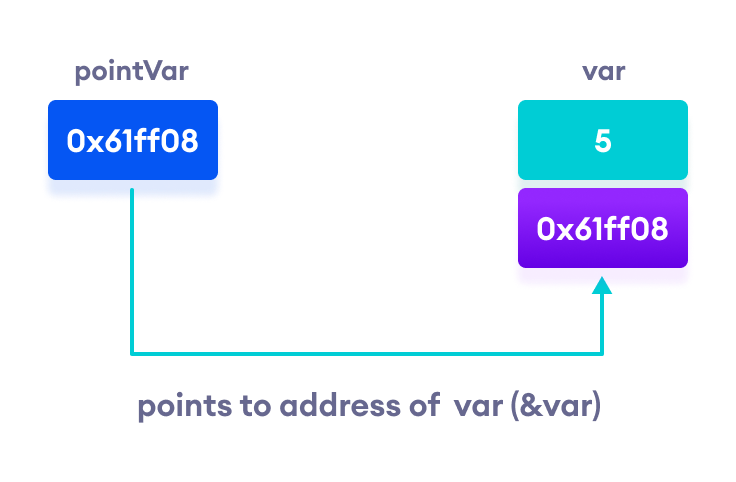
\includegraphics[width=4in]{images/cpp-pointer-working.png}
\caption{Working of C++ pointers}
\end{figure}

\doublelinewithspace{.0cm}

\hypertarget{changing-value}{%
\subsubsection{Changing Value Pointed by Pointers}\label{changing-value}}

If \texttt{pointVar} points to the address of \texttt{var}, we can
change the value of \texttt{var} by using \texttt{*pointVar}.

\textbf{For example,}
\begin{minted}[linenos]{c++}
int var = 5;
int* pointVar;

// assign address of var
pointVar = &var;

// change value at address pointVar
*pointVar = 1;

cout << var << endl; // Output: 1
\end{minted}

Here, \texttt{pointVar} and \texttt{\&var} have the same address, the
value of \texttt{var} will also be changed when \texttt{*pointVar} is
changed.

\doublelinewithspace{.0cm}

\hypertarget{example3}{%
\subsubsection{Example 3: Changing Value Pointed by
Pointers}\label{example3}}

\begin{minted}[linenos]{c++}
#include <iostream>
using namespace std;
int main() {
    int var = 5;
    int* pointVar;

    // store address of var
    pointVar = &var;

    // print var
    cout << "var = " << var << endl;

    // print *pointVar
    cout << "*pointVar = " << *pointVar << endl
         << endl;

    cout << "Changing value of var to 7:" << endl;

    // change value of var to 7
    var = 7;

    // print var
    cout << "var = " << var << endl;

    // print *pointVar
    cout << "*pointVar = " << *pointVar << endl
         << endl;

    cout << "Changing value of *pointVar to 16:" << endl;

    // change value of var to 16
    *pointVar = 16;

    // print var
    cout << "var = " << var << endl;

    // print *pointVar
    cout << "*pointVar = " << *pointVar << endl;
    return 0;
}
\end{minted}

\textbf{Output}
\begin{minted}[bgcolor=bg]{text}
var = 5
*pointVar = 5

Changing value of var to 7:
var = 7
*pointVar = 7

Changing value of *pointVar to 16:
var = 16
*pointVar = 16
\end{minted}

\doublelinewithspace{.0cm}

\hypertarget{common-mistakes}{%
\subsection{Common mistakes when working with pointers}\label{common-mistakes}}

Suppose, we want a pointer \texttt{varPoint} to point to the address of \texttt{var}. Then,

\begin{minted}[linenos]{c++}
int var, *varPoint;

// Wrong! 
// varPoint is an address but var is not
varPoint = var;

// Wrong!
// &var is an address
// *varPoint is the value stored in &var
*varPoint = &var;

// Correct! 
// varPoint is an address and so is &var
varPoint = &var;

 // Correct!
// both *varPoint and var are values
*varPoint = var;
\end{minted}

% \doublelinewithspace{.0cm}

% \textbf{Recommended Readings}:

% \begin{itemize}
% \tightlist
% \item
%   \href{/cpp-programming/pointer-void}{How to use generic data type
%   pointers using a void pointer?}
% \item
%   \href{/cpp-programming/pointers-arrays}{How to represent an array
%   using a pointer?}
% \item
%   \href{/cpp-programming/pointers-function}{How to use pointers with
%   functions?}
% \item
%   \href{/cpp-programming/structure-pointer}{How to use pointers with
%   structures?}
% \end{itemize}

% \href{/cpp-programming/operator-overloading}{}

